\documentclass{article}

\usepackage{fancyhdr, lastpage}
\usepackage[inline]{enumitem}
\usepackage{listings}
\usepackage[scaled=0.95]{inconsolata}  % Use a monospaced font, like Inconsolata
\usepackage{wasysym}
\usepackage{booktabs}
\usepackage{booktabs, multicol, multirow, array, threeparttable}
\usepackage{siunitx}
\usepackage{xfrac}
\usepackage{extramarks}
\usepackage{amsmath, amsthm, amsfonts, mathtools, empheq}
\usepackage{caption}
\usepackage[table]{xcolor}
\usepackage{tikz}
\usepackage[most]{tcolorbox}
\usepackage{pagecolor} %% for dark background
\usepackage{hyperref}
\usepackage{refcount}
\usepackage{subfigure}

\topmargin=-0.45in
\evensidemargin=0in
\oddsidemargin=0in
\textwidth=6.5in
\textheight=9.0in
\headsep=0.25in

\linespread{1.1}

% Define a command to print last page number without hyperlink
\newcommand*{\lastpagewithoutlink}{%
    \getpagerefnumber{LastPage}%
}

\pagestyle{fancy}
\lhead{\hmwkAuthorName}
\chead{\hmwkTitle}
\rhead{\hmwkClass}
\lfoot{\lastxmark}
\cfoot{Page \thepage \ of \lastpagewithoutlink}


\renewcommand\headrulewidth{0.4pt}
\renewcommand\footrulewidth{0.4pt}

\setlength\parindent{0pt}

%
% Create Problem Sections
%

\newcommand{\enterProblemHeader}[1]{
    \nobreak\extramarks{}{Problem \arabic{#1} continued on next page\ldots}\nobreak{}
    \nobreak\extramarks{Problem \arabic{#1} (continued)}{Problem \arabic{#1} continued on next page\ldots}\nobreak{}
}

\newcommand{\exitProblemHeader}[1]{
    \nobreak\extramarks{Problem \arabic{#1} (continued)}{Problem \arabic{#1} continued on next page\ldots}\nobreak{}
    \stepcounter{#1}
    \nobreak\extramarks{Problem \arabic{#1}}{}\nobreak{}
}

\setcounter{secnumdepth}{0}
\newcounter{partCounter}
\newcounter{homeworkProblemCounter}
\setcounter{homeworkProblemCounter}{1}
\nobreak\extramarks{Problem \arabic{homeworkProblemCounter}}{}\nobreak{}

%
% Homework Problem Environment
%
% This environment takes an optional argument. When given, it will adjust the
% problem counter. This is useful for when the problems given for your
% assignment aren't sequential. See the last 3 problems of this template for an
% example.
%
\newenvironment{homeworkProblem}[1][-1]{
    \ifnum#1>0
        \setcounter{homeworkProblemCounter}{#1}
    \fi
    \section{Problem \arabic{homeworkProblemCounter}}
    \setcounter{partCounter}{1}
    \enterProblemHeader{homeworkProblemCounter}
}{
    \exitProblemHeader{homeworkProblemCounter}
}

%
% Homework Details
%   - Title
%   - Due date
%   - Class
%   - Section/Time
%   - Instructor
%   - Author
%

\newcommand{\hmwkTitle}{Homework\ \#6}
\newcommand{\hmwkDueDate}{May 15th, 2024}
\newcommand{\hmwkClass}{EGR 5110}
\newcommand{\hmwkClassTime}{}
\newcommand{\hmwkClassInstructor}{Professor Nissenson}
\newcommand{\hmwkAuthorName}{\textbf{Francisco Sanudo}}

%
% Title Page
%

\title{
    \vspace{2in}
    \textmd{\textbf{\hmwkClass:\ \hmwkTitle}}\\
    \normalsize\vspace{0.1in}\small{Due\ on\ \hmwkDueDate\ at 11:59pm}\\
    \vspace{0.1in}\large{\textit{\hmwkClassInstructor\ \hmwkClassTime}}
    \vspace{3in}
}

\author{\hmwkAuthorName}
\date{}

\renewcommand{\part}[1]{\textbf{\large Part \Alph{partCounter}}\stepcounter{partCounter}\\}

%
% More settings
%

% Define MATLAB code style
\lstdefinestyle{matlabstyle}{%
  language=Matlab,
  basicstyle=\ttfamily\small,    % Use a smaller font
  keywordstyle=\color{blue},
  commentstyle=\color{green!40!black},
  stringstyle=\color[RGB]{167, 9, 245},
  numbers=left,
  numberstyle=\tiny,
  numbersep=5pt,
  frame=single,
  breaklines=true,
  breakatwhitespace=true,
  captionpos=b,
  morekeywords={matlab2tikz},
  showstringspaces=false,
}

\newcommand{\mat}[1]{\lstinline[style=matlabstyle]|#1|}

% Table Settings
% \setlength{\tabcolsep}{5pt} % Gap before text starts
\renewcommand{\arraystretch}{2.5} % Cell Height Scaling
\setlength{\arrayrulewidth}{0.5mm} % Table Border Thickness
\arrayrulecolor{blue} % Table Border Color
\newcolumntype{s}{>{\columncolor{black!10}} c}

% Link Settings
\hypersetup{
    colorlinks=false,       % false: boxed links; true: colored links
    linkcolor=red,          % color of internal links (change box color with linkbordercolor)
    citecolor=green,        % color of links to bibliography
    urlcolor=cyan,           % color of external links
    pdftitle={EGR 5110 HW3}
}

% Color defintions
\definecolor{magenta}{RGB}{255,0,255}
\definecolor{cyan}{RGB}{0,255,255}
\definecolor{white}{RGB}{255,255,255}
\definecolor{red}{RGB}{255,0,0}
\definecolor{green}{RGB}{0,255,0}
\definecolor{orange}{RGB}{255,165,0}
\definecolor{yellow}{RGB}{255,255,0}
\definecolor{blue}{RGB}{10,10,255}

% Text color shortcuts
\newcommand{\cw}{\color{white}}
\newcommand{\cm}{\color{magenta}}
\newcommand{\cc}{\color{cyan}}
\newcommand{\cred}{\color{red}}
\newcommand{\cb}{\color{blue}}
\newcommand{\cg}{\color{green}}
\newcommand{\cy}{\color{yellow}}
\newcommand{\co}{\color{orange}}

%
% Various Helper Commands
%


% For derivatives
\newcommand{\deriv}[2]{\frac{d#1}{d#2}}

% For partial derivatives
\newcommand{\pderiv}[2]{\displaystyle \frac{\partial #1}{\partial #2}}

% Redefine \dfrac if you want all fractions to be in display style automatically
\newcommand{\ddfrac}[2]{\frac{\displaystyle #1}{\displaystyle #2}}

% Alias for the Solution section header
\newcommand{\solution}{\textbf{\large Solution}}

%% Box settings
% \setlength{\fboxsep}{9pt} % Adjust the padding thickness here
\setlength{\fboxrule}{1pt} % Adjust the border thickness here

% The \dimexpr\linewidth-2\fboxsep-2\fboxrule\relax calculation ensures that the width of the minipage is reduced by twice the padding and twice the border width, as there is padding and border on both the left and right sides.
\newcommand{\boxsettings}{\dimexpr\linewidth-2\fboxsep-2\fboxrule\relax}

% Paragraph box shortcut for tables
\newcommand{\PB}[2]{\parbox{#1}{\centering #2}}

%% make subscripts smaller
% \begingroup\lccode`~=`_
% \lowercase{\endgroup\def~}#1{_{\scriptscriptstyle#1}}
% \AtBeginDocument{\mathcode`_="8000 \catcode`_=12 }

%% small negative sign
\newcommand{\dashexp}{\scalebox{0.35}[0.5]{$-$}}
\newcommand{\dash}{\scalebox{0.5}[1.0]{$-$}}


\begin{document}

\maketitle

\pagebreak

\tableofcontents

\pagebreak

\section{Background: Optimization and Gradient Ascent with Backtracking Line Search}

Optimization is a fundamental problem in mathematics and computer science, where the goal is to find the best solution (maximum or minimum) of an objective function within a given domain. In numerical methods, optimization algorithms are employed to efficiently navigate through the solution space and locate optimal points.

\subsection{Objective Function}
Consider an objective function \( f(x, y) \) representing a scalar-valued function of two variables \( x \) and \( y \). The goal of optimization is to maximize \( f(x, y) \) with respect to \( (x, y) \) within a specified region.

\subsection{Gradient Ascent}
Gradient ascent is an iterative optimization algorithm used to maximize a function by following the direction of steepest ascent of the gradient. The gradient \( \nabla f(x, y) \) at a point \( (x, y) \) points in the direction of the greatest rate of increase of \( f \). Therefore, moving in the direction of the gradient can lead to local maxima of the function.

\subsection{Backtracking Line Search}
Backtracking line search is a technique used in optimization to determine an appropriate step size for gradient-based methods. Instead of using a fixed step size, backtracking line search dynamically adjusts the step size based on certain criteria, ensuring that the function value increases sufficiently in the direction of the gradient.

\subsection{Armijo Condition}
The Armijo condition is a key component of backtracking line search. It ensures that the function value decreases sufficiently with respect to the gradient direction and the chosen step size. The Armijo condition is typically expressed as:
\[
f(x + h \cdot g) \leq f(x) + \sigma \cdot h \cdot (g^T g)
\]
where \( h \) is the step size, \( g \) is the gradient vector, \( \sigma \) is a small constant (e.g., \( 0 < \sigma < 1 \)), and \( g^T g \) denotes the squared norm of the gradient.

\subsection{Armijo Condition vs. Exact Line Search}
The Armijo condition is preferred over exact line search methods for several reasons:
\begin{itemize}
    \item \textbf{Computational Efficiency}: Exact line search methods require costly evaluations of the objective function, especially in high-dimensional spaces. In contrast, the Armijo condition only requires a few function evaluations to determine a suitable step size.
    \item \textbf{Robustness}: The Armijo condition provides a balance between ensuring sufficient decrease in the function value and avoiding excessive computation associated with exact line search methods.
    \item \textbf{Adaptability}: Backtracking line search with the Armijo condition can handle noisy or ill-conditioned objective functions more effectively compared to exact line search methods.
\end{itemize}

\section{Gradient Ascent Algorithm in MATLAB}
Homework \#5 required the implementation of a the gradient ascent algorithm with inexact (backtracking) line search  to solve a 2D unconstrained optimization problem. Here's a brief explanation of the key components and flow of the code, which can be found in Listing \ref{lst:calcMaxStudent}:

\subsection{Inputs}
\begin{itemize}
    \item \mat{f} --  Objective function (anonymous function of x and y)
    \item \mat{xi \& yi} -- Initial guesses for x and y
    \item \mat{tol} -- Error tolerance for convergence
    \item \mat{sigma} -- Armijo condition constant
    \item \mat{beta} -- Backtracking constant
\end{itemize}

\subsection{Outputs}
\begin{itemize}
    \item \mat{xypos} --  Array containing the (x, y) coordinates at each step
    \item \mat{numsteps} -- Number of steps required for convergence
    \item \mat{numfneval} -- Number of function evaluations
\end{itemize}

\subsection{Optimization Process}
\begin{enumerate}
    \item Inititialization
        \begin{itemize}
            \item Set initial parameters (\mat{numsteps}, \mat{numfneval}, \mat{maxiter}, \mat{converged}).
            \item Initialize the current position \mat{X} with the initial guesses.
        \end{itemize}
    \item Gradient Ascent with Backtracking Line Search
        \begin{itemize}
            \item Iterate until convergence (\mat{converged = true}) or maximum iterations (\mat{maxiter}) are reached.
            \item Compute the gradient \mat{g} of the function at the current position \mat{X}.
            \item Check the convergence condition based on the gradient norm (\mat{err < tol}).
            \item Implement backtracking line search using the Armijo condition to ensure a sufficient decrease in the function value.
            \item Update the position \mat{X} based on the computed step size (\mat{h}) and the gradient direction.
            \item Record the updated position in \mat{xypos}.
        \end{itemize}
    \item Contour Plot
        \begin{itemize}
            \item After optimization, visualize the path taken (\mat{xypos}) overlaid on the contour plot of the function.
            \item Evaluate the function \mat{f} over a grid of \mat{x} and \mat{y} values to create the contour plot.
            \item Plot the starting point (\mat{xi}, \mat{yi}), the path (\mat{xypos}), an the optimal solution (\mat{xypos(end,1)}, \mat{xypos(end,2)})
        \end{itemize}
\end{enumerate}

\subsection{Utility Functions}
\begin{itemize}
    \item \mat{grad}: Estimates the gradient of \mat{f} using central finite-difference approximation.
    \item \mat{euclideanNorm}: Computes the Euclidean norm of a vector.
    \item \mat{applyFigureProperties}: Configures figure properties for plotting.
\end{itemize}

\subsection{Recommendations}
\begin{itemize}
    \item Ensure the objective \mat{f} is well-defined and behaves appropriately for the optimization task.
    \item Tune the parameters (\mat{tol}, \mat{sigma}, \mat{beta}, \mat{maxiter}) based on the characteristics of the objective function.
    \item Verify the gradient approximation (\mat{grad}) accuracy with a smaller perturbation (\mat{delta}) if needed.
    \item To find a local minima (i.e. gradient descent), simply negate the sign of the gradient when updating the position at each step, and also modify the Armijo condition to ensure that the function \textbf{decreases} by a minimum amount at each step.
\end{itemize}

\section{Simulations}
Consider the set of input parameters specified for the optimization algorithm using gradient ascent with backtracking line search. Each scenario is defined by different values of tolerance (tol), Armijo condition constant ($\sigma$), and backtracking constant ($\beta$). The objective function $f(x,y)$ and initial guesses for $x$ and $y$ are also specified.
\\

Here is an example of how the inputs are defined for the base case:
\begin{lstlisting}[style=matlabstyle, caption = {Function Inputs}]
xi = -10; yi = 5;                               % initial guesses
f = @(x,y) -10*(x-2).^2 - 5*(y+3).^2 + 20;      % objective function
tol = 0.01;                                     % tolerance
sigma = 0.0001;                                 % armijo condition consant
beta = 0.5;                                     % backtracking constant
\end{lstlisting}

\subsection{Objective function and Optimization Setup}
The objective function $f(x,y) = -10(x-2)^2 - 5(y+3)^2 + 20$ represents a quadratic function with a known maximum. The goal is to find the local maximum of $f(x,y)$ starting from the initial guesses $X_i=-10$ and $y_i=5$.

\begin{table}[t]
    \centering
    \caption{Ten Scenarios Demonstrating Effects of Varying tol, $\sigma$, and $\beta$}
    \small
    \begin{tabular}{|s|c|c|c|c|c|} \hline
        {\cellcolor{yellow!50} \bf Scenario} & {\PB{1.6cm}{tol}}    & {\PB{1.6cm}{$\sigma$}} & {\PB{1.6cm}{$\beta$}}  & {\PB{1.6cm}{Steps}} & {\PB{1.6cm}{Function\\ evaluations}}
        \\ \hline
        1       & 0.01     & 0.0001     & 0.5    &  11  & 93    \\ \hline
        $2^*$   & 0.01     & 0.0001     & 0.9    &  328 & 8834  \\ \hline
        3       & 0.01     & 0.0001     & 0.1    &  48  & 333   \\ \hline
        4       & 0.01     & 0.0001     & 0.01   &  87  & 521   \\ \hline
        5       & 0.01     & 0.01       & 0.5    &  11  & 93    \\ \hline
        6       & 0.01     & 0.1        & 0.5    &  10  & 85    \\ \hline
        $7^*$   & 0.01     & 0.9        & 0.5    &  64  & 716   \\ \hline
        8       & 1e\dash1 & 0.0001     & 0.5    &  9   & 76    \\ \hline
        9       & 1e\dash4 & 0.0001     & 0.5    &  15  & 129   \\ \hline
        $10^*$  & 1e\dash6 & 0.1        & 0.5    &  19  & 164   \\ \hline
    \end{tabular}
    \label{tab:Scenarios}
\end{table}


\subsection{Scenarios}
Table \ref{tab:Scenarios} presents ten simulation scenarios with varying parameter values (tol, $\sigma$, $\beta$) and corresponding results from the optimization algorithm.

\begin{itemize}
    \item \textbf{Steps}: Number of iterations required to reach convergence (within the specified tolerance).
    \item \textbf{Function Evaluations}: Total number of function evaluations performed during optimization.
\end{itemize}

Noteworthy scenarios marked with an asterisk (*) indicate that a plot was generated and the results are discussed further in the Results section.

\pagebreak

\subsection{Intepretation of Results}
The output from the optimization algorithm (Listing \ref{lst:output}) for the base case (scenario 1) provides insights into the optimization process:

\begin{itemize}
    \item \textbf{Optimal Point}: The coordinates $(x,y)$ of the local maximum identified by the alogrithm (shown at the final step if convergence is reached).
    \item \textbf{Iterative Process}: Sequence of points $(x,y)$ visited during the optimization iterations, captured in the \mat{xypos} array.
    \item \textbf{Algorithm Performance}:
        \begin{itemize}
            \item \textbf{Number of Steps}: Indicates the convergence behavior of the algorithm.
            \item \textbf{Function Evaluations}: Reflects the computational cost in terms of objective function evaluations.
        \end{itemize}
\end{itemize}

\pagebreak

\begin{lstlisting}[style=matlabstyle, caption = {Optimization Algorithm Output},numbers=none, label={lst:output}]
>> [xypos,numsteps,numfneval] = calcMaxStudent(f,xi,yi,tol,sigma,beta);

Results:
       x         y
  -10.0000    5.0000
    5.0000   -0.0000
    1.2500   -1.8750
    2.1875   -2.5781
    1.7188   -3.1055
    2.0703   -3.0396
    1.9824   -3.0148
    2.0044   -3.0056
    1.9989   -3.0021
    2.0016   -2.9995
    1.9996   -2.9998


Number of steps = 11
Number of function evaluations = 93
\end{lstlisting}

\subsection*{Discussion of Key Scenarios}

In this section, we delve into the results and insights gained from the simulations of scenarios 2*, 7*, and 10*.

\subsubsection*{Scenario 2*}

Scenario 2* utilized a small tolerance (\( \text{tol} = 0.01 \)) and a high backtracking constant (\( \beta = 0.9 \)). This combination resulted in a large number of steps (328) and function evaluations (8834) when compared to scenario 1. The optimization algorithm with these parameters displayed a cautious approach, taking smaller steps towards the local maximum due to the significant backtracking. The plot generated for this scenario, seen in Figure \ref{fig:scenario2}, shows a detailed path towards convergence, indicating careful adjustment of the step size at each iteration.

\subsubsection*{Scenario 7*}

In scenario 7*, a higher Armijo condition constant (\( \sigma = 0.9 \)) was employed along with standard tolerance (\( \text{tol} = 0.01 \)) and backtracking constant (\( \beta = 0.5 \)). Despite the larger \( \sigma \), the algorithm required 64 steps and 716 function evaluations to converge. This behavior suggests that while a higher \( \sigma \) allows larger steps, it may also necessitate more cautious adjustments during the line search process. Figure \ref{fig:scenario7} illustrates the optimization path, showcasing the impact of the armijo condition on step size decisions.

\subsubsection*{Scenario 10*}

Scenario 10* explored a scenario with an extremely small tolerance (\( \text{tol} = 1 \times 10^{-6} \)) and a higher Armijo condition constant (\( \sigma = 0.1 \)). These parameters facilitated convergence in 19 steps with 164 function evaluations. The small tolerance forced the algorithm to meticulously approach the maximum, while the moderate \( \sigma \) allowed more substantial steps compared to other scenarios with similar tolerances. Figure \ref{fig:scenario10} illustrates the optimization journey, emphasizing the balance between precision and computational efficiency.

\pagebreak

\begin{figure}[h]
    \centering
    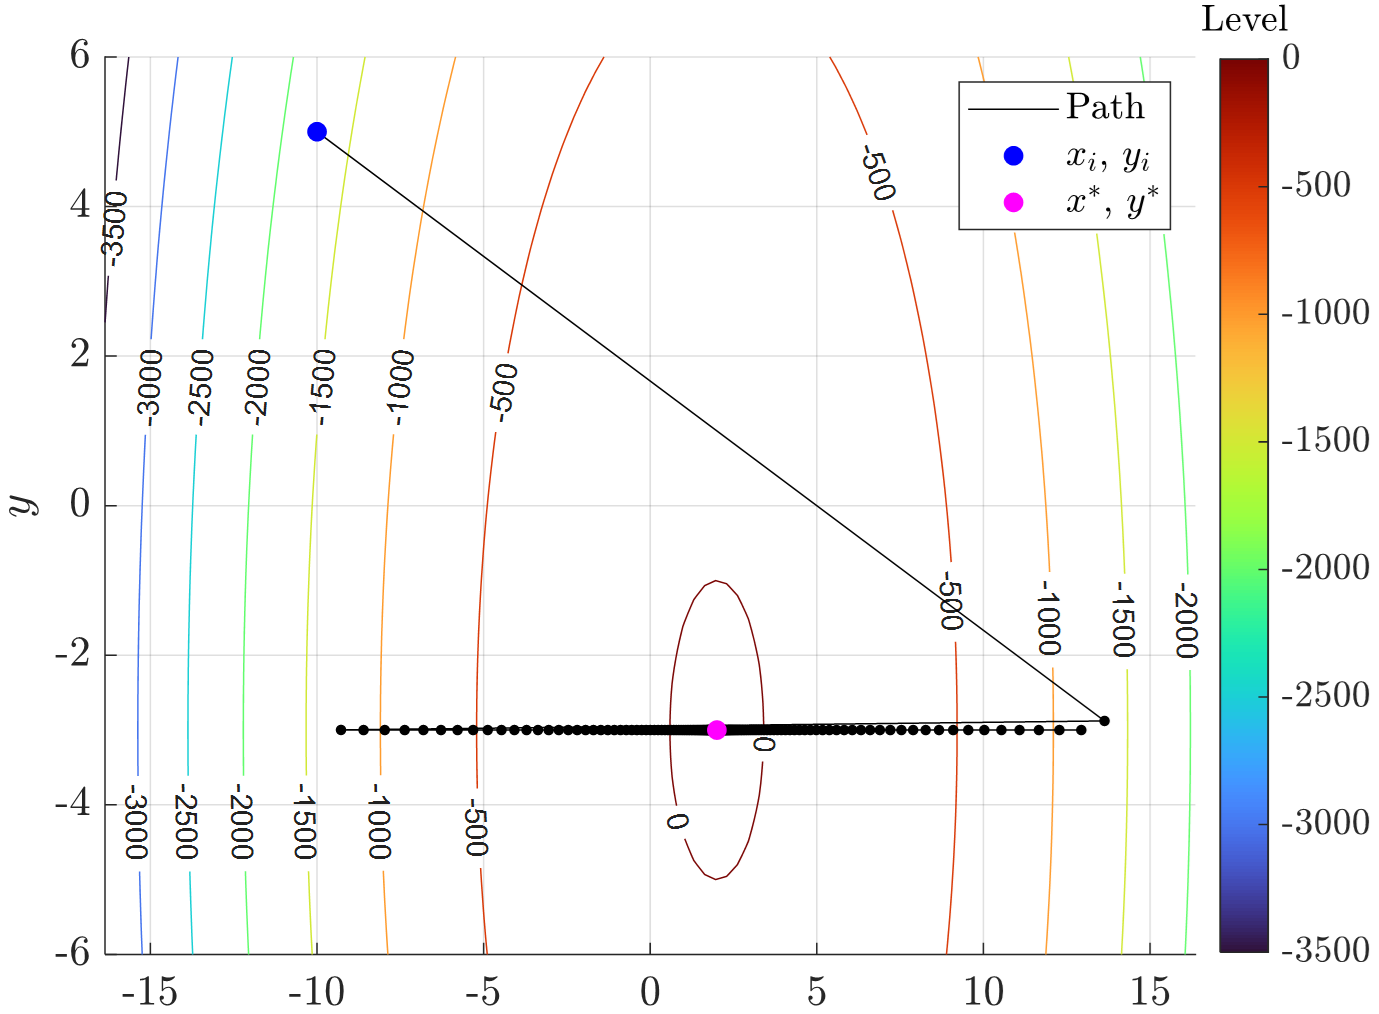
\includegraphics[width = 0.47\textwidth]{fig/scenario2.png}
    \caption{Optimization Path for Scenario 2}
    \label{fig:scenario2}
\end{figure}

\begin{figure}[h]
    \centering
    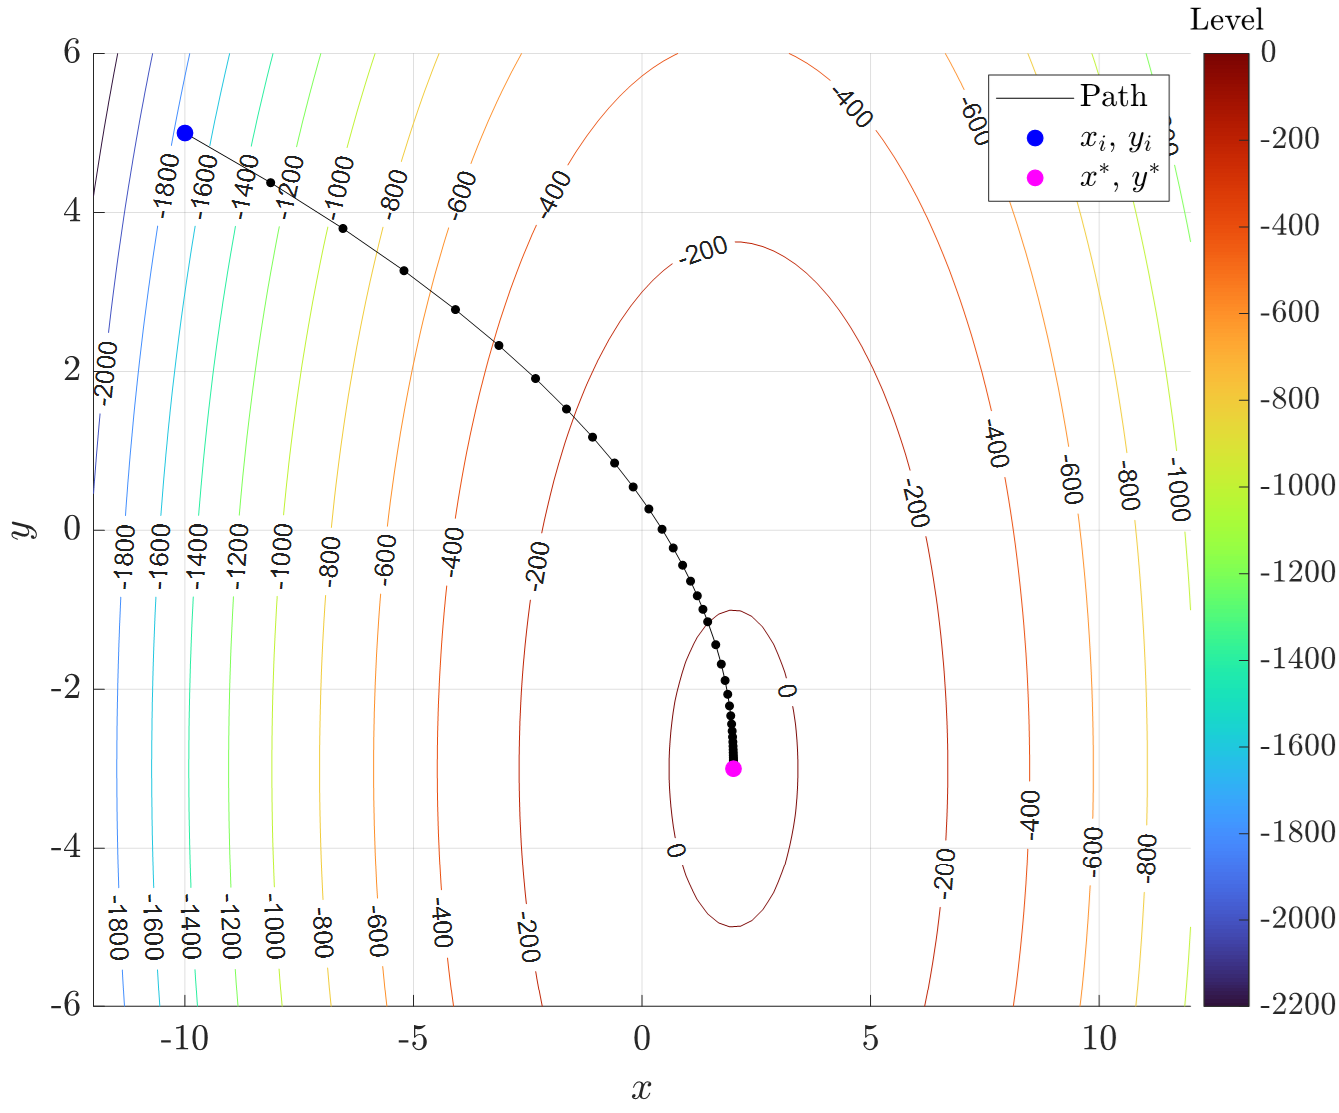
\includegraphics[width = 0.47\textwidth]{fig/scenario7.png}
    \caption{Optimization Path for Scenario 7}
    \label{fig:scenario7}
\end{figure}

\begin{figure}[h!]
    \centering
    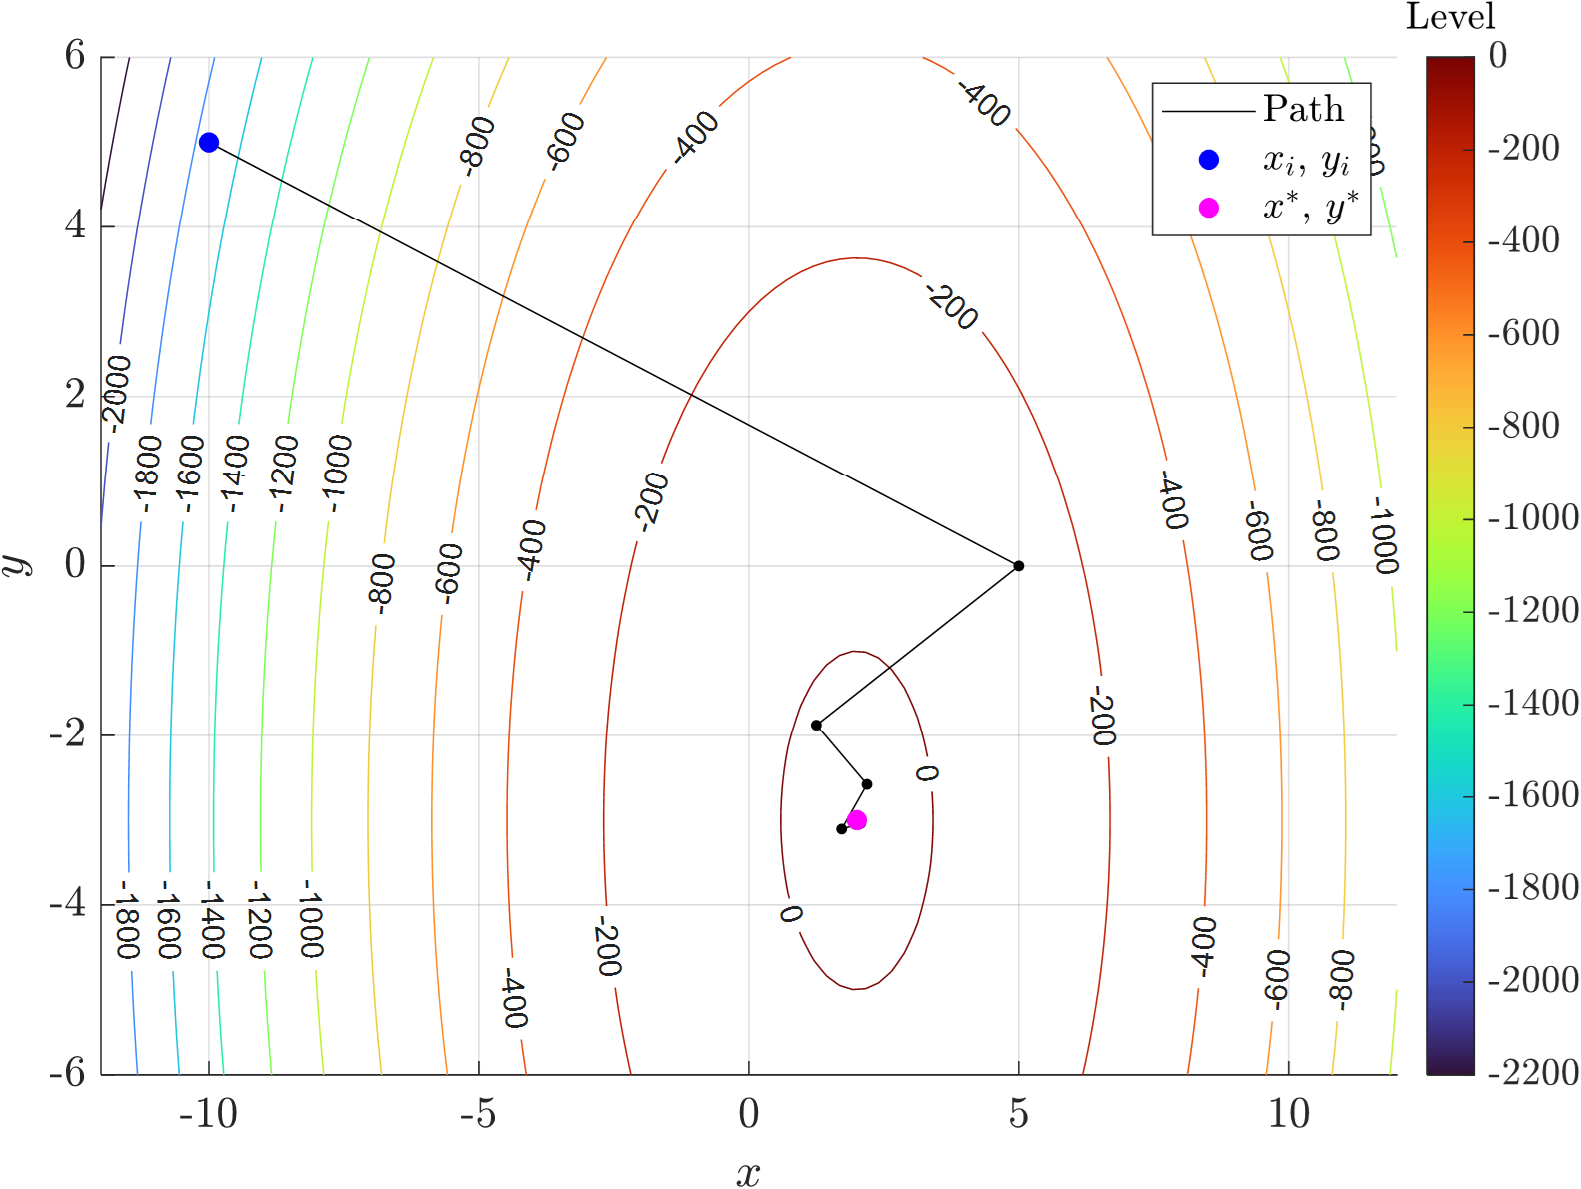
\includegraphics[width = 0.47\textwidth]{fig/scenario10.png}
    \caption{Optimization Path for Scenario 10}
    \label{fig:scenario10}
\end{figure}

\pagebreak

\section{MATLAB Code}

\lstinputlisting[
  style=matlabstyle,
  caption={Gradient Ascent Algorithm with Inexact (Backtracking) Line Search for 2D Optimization},
  label={lst:calcMaxStudent}
]{../code/calcMaxStudent.m}

\end{document}
